\documentclass[12pt]{exam}
\newcommand{\hwnumber}{7}
\newcommand{\hwname}{Bloom Filters}
\newcommand{\duedate}{\formatdate{21}{03}{\YEAR} by \progDueTime}

\usepackage{../misc/latex/edition}  % Course semester
\usepackage{../misc/latex/c0}       % Listings style for c0
\usepackage{amsmath}
\usepackage{enumerate}
\usepackage[normalem]{ulem}
\usepackage{verbatim}
\usepackage[left=1in, right=1in, top=1in, bottom=1in]{geometry}
\usepackage{graphicx}
\usepackage{hyperref}
\usepackage{tikz}     \usetikzlibrary{shapes}
\usepackage{fancybox}
\usepackage[all]{xy}
\usepackage{wrapfig}
\usepackage{fancyvrb}
\usepackage{datetime}
\usepackage{etoolbox}
\usepackage{calc}
\usepackage[nomessages]{fp}
\usepackage{import}  % Like input and include, but respects subdirectories

\newcommand{\defaultQuestionLocation}{questions}
\newcommand{\inputQuestion}[2][\defaultQuestionLocation/]{%
  \subimport{#1}{#2}
}
% Subdirectories of \defaultQuestionLocation containing code and pictures
\newcommand{\code}{code}
\newcommand{\img}{img}


%%% ic: frontmatter macros
\newcommand{\specialInstructions}{}
\newcommand{\HWNUMBER}
{\ifdefempty{\hwnumber}{__}{%
  \ifnumless{\hwnumber}{10}{0\hwnumber}{\hwnumber}}}
\newcommand{\hwtype}{Written Homework}

%%% ic: 'exam' tweaks
\renewcommand{\half}{.5} % Half points

\newcommand{\Question}[2][]
 {\ifstrempty{#1}
    {\question{\bf #2}}
    {\question[#1]{\bf #2}}
  \immediate\write\rubricfile{}%
  \immediate\write\rubricfile{Question \thequestiontitle:}%
  \immediate\write\rubricfile{==========}
 }

%%% ic: Support for editable PDF
% counter name (some viewers misbehave if always the same)
\newcounter{editable}
\newcommand{\nextField}{\addtocounter{editable}{1}q\arabic{editable}}
\newcommand{\NextField}
 {\makebox[0pt][r]{\scalebox{0.1}{\color{White}\nextField}}}

% Color of edit area
\newcommand{\editAreaColor}{red}
% Single line answer:   \editableLine[extra parameters (optional)]{line width}
\newcommand{\editableLine}[2][]
{\textcolor{\editAreaColor}{%
 \underline{\hspace*{-0.25em}%
 \raisebox{-0.5ex}{%
 \TextField[width=#2, borderwidth=0, #1]{\NextField}}}}%
}
% Single line answer for code:  \editableLine[extra parameters (optional)]{line width}
\newcommand{\editableCodeLine}[2][]
{\textcolor{\editAreaColor}{%
 \underline{%
 \TextField[width=#2, height=1.5ex, borderwidth=0, #1]{\NextField}}}}
% Multiline answer:  \editableLine[extra parameters (optional)]{box height}
\newcommand{\editableBox}[2][]
{\leavevmode\hspace*{-0.1em}%
\TextField[height=#2, width=\linewidth,
           multiline=true, borderwidth=0.1, bordercolor=\editAreaColor,
           #1]{\NextField}}

%%%%% Same answer format as exams
\renewcommand{\rmdefault}{ppl}
\renewcommand{\sfdefault}{phv}
\newcommand{\answerColor}{Blue}

\ifprintanswers
\newcommand{\answer}[2]{\makebox[#1][c]{\color{\answerColor}#2}}
\else
\newcommand{\answer}[2]{\makebox[#1][c]{}\makebox[0pt]{\phantom{|}}}
\fi
\newcommand{\uanswer}[2]{\underline{\answer{#1}{#2}}}


%%% Write rubric snippet.  Usage:
% \RUBRIC
% any multi-line text (including \, #, %, whatever)
% ENDRUBRIC
%% (ENDRUBRIC should be on a line by itself)
\makeatletter
\def\RUBRIC
 {%
  \begingroup
  \let\do\@makeother\dospecials
  \endlinechar=`\^^J
  \@tofile%
 }
\def\ENDRUBRIC{ENDRUBRIC}
\def\@tofile#1^^J{%
  \def\@test{#1}%
  \ifx\@test\ENDRUBRIC
    \immediate\write\rubricfile{}  % End with an empty line
    \expandafter\@firstoftwo
  \else
    \expandafter\@secondoftwo
  \fi
  {\endgroup}%
  {\toks@{#1}%
   \begingroup\endlinechar=\m@ne
   \everyeof{\noexpand}%
   \xdef\@temp{\scantokens\expandafter{\the\toks@}}%
   \endgroup
   \immediate\write\rubricfile{\@temp}%
   \@tofile}%
}
\makeatother

%% Displays tags for an exercise in 'answer' mode
\newcommand{\TAGS}[1]
{\ifprintanswers%
  \rule{0em}{0ex}%
  \marginpar{\footnotesize%
    \fcolorbox{black}{Gray!25}{%
      \parbox[t]{2cm}{\raggedright\textbf{TAGS:}\\#1}}}%
  \ignorespaces%
 \fi}%


%% Page layout
\pagestyle{headandfoot}

\headrule
\header{\textbf{\courseNumber{} \hwtype{} \hwnumber}}
       {}
       {\textbf{Page \thepage\ of \numpages}}
\footrule
\footer{}{}{\COPYRIGHT}

\renewcommand{\partlabel}{\textbf{\thequestion.\thepartno}}
%\renewcommand{\partlabel}{\textbf{Task \thepartno}}
\renewcommand{\subpartlabel}{\textbf{\thesubpart.}}
\renewcommand{\thepartno}{\arabic{partno}}
\renewcommand{\thesubpart}{\alph{subpart}}
\pointpoints{pt}{pts}
\pointformat{\raisebox{0ex}[\height][0pt]{\fcolorbox{black}{yellow}{\themarginpoints}}}
\bonuspointformat{\raisebox{0ex}[\height][0pt]{\fcolorbox{black}{red}{\themarginpoints}}}
\marginpointname{\points}
\pointsinmargin
%\boxedpoints

\setlength\answerlinelength{2in}
\setlength\answerskip{0.3in}

\newcommand{\mkWrittenTitle}[1]{#1}
\newcommand{\mkDueDate}[1]{#1}
\newcommand{\mkEvalSummary}[1]{#1}
\newcommand{\mkGradetable}[1]{#1}



% This fixes an issue with the exam package version 2.6 and after,
% where 'framed' has been renamed to 'examframed' to avoid a conflict.
\ifcsmacro{examframed}{%
\newenvironment{framed}
{\begin{examframed}}
{\end{examframed}}
}{}

\usepackage{pifont}
\begin{document}
\hwTitle

\noindent
In this assignment, you will implement a variation of hash-table-based
sets, called \emph{Bloom filters}, and explore some of the
applications of Bloom filters.  The code handout for this assignment
is on \autolab{} and at
\begin{center}
\whereisthetgz{bloom-handout.tgz}
\end{center}
The file \lstinline'README.txt' in the code handout goes over the contents
of the handout and explains how to hand the assignment in.  There is
a FIVE (5) PENALTY-FREE HANDIN LIMIT.
Every additional handin will incur a small (5\%) penalty (even if
using a late day).

To help you write test cases for Task 1, which we want you to
do before starting on the later tasks, there will be a separate, unofficial
``Bloom Filter Test Case Checker'' Autolab assignment. This will
only run the part of the autograder that checks
Task 1. There is no handin limit for that unofficial
autograder. Check the \lstinline'README.txt' file carefully for details.

\section{Bloom Filters}

Fundamentally, Bloom filters are an implementation of the \emph{set
  interface} discussed in the lecture handout:
\begin{quote}
\begin{lstlisting}
// typedef ______* bloom_t;

bloom_t bloom_new(int capacity)
  /*@requires capacity > 0; @*/
  /*@ensures \result != NULL; @*/ ;

bool bloom_contains(bloom_t B, string x)
  /*@requires B != NULL; @*/ ;

void bloom_add(bloom_t B, string x)
  /*@requires B != NULL; @*/
  /*@ensures bloom_contains(B, x); @*/ ;
\end{lstlisting}
\end{quote}
The one interesting twist is that the \lstinline'bloom_contains' function
\emph{is allowed to return false positives}. If the Bloom filter says that
something \emph{is not} in the set, it has to be right, but if it says that
something \emph{is} in the set, it can be wrong. To put it a different way,
a Bloom filter answers the question ``is \lstinline'x' in the set?'' with
either the answer ``no'' or ``maybe.''

Try to think of a couple of obvious and possibly silly ways you could
implement this interface before you turn the page.


\clearpage

There are a lot of possible correct implementations of the interface we gave
on the previous page.  One always returns \lstinline'true', signaling
``maybe \lstinline'x' is in the set.'' You've been provided with this
implementation in \lstinline'bloom-worst.c0', and it is, according to the
description we gave, a \emph{correct} implementation. It is also very fast
and uses very little space!  It is terrible in every other possible way.

At the other end of the spectrum, you could implement a proper set. You have
the tools to do this in a couple of ways: unbounded arrays (sorted or not),
linked lists, and hash tables. You have been provided with one such
implementation in \lstinline'bloom-expensive.c0'. Such an implementation will
only signal ``maybe \lstinline'x' is in the set'' when \lstinline'x' is
\emph{really, actually} in the set. This is fine, but it ends up using lots of
memory, and what's more, the implementation you were given is quite slow.

The implementations we're going to explore in this assignment will be
in-between: they use less memory than a real hash table, but give
fewer false positives than a completely non-committal
implementation. Before we talk about how to do this, and before we go
and do it, let's write some tests!

\subsection{Testing Bloom Filters}

\begin{task}[6]
\TAGS{testing}
Write a testing program \lstinline'bloom-test.c0' that respects the
interface on the previous page. It should serve two purposes:
\begin{itemize}
\item%
  The testing program should attempt to raise an assertion error on any
  incorrect implementation of the interface.
\item%
  On any correct implementation of the Bloom filter interface, the
  \lstinline'main()' function should return a \emph{performance score} from 0
  and 100 (inclusive).
  \begin{itemize}
    \item On the worst possible Bloom filter implementation described
      above, the performance score should be 0.
    \item On an ``error free'' Bloom filter implementation (such as an
      actual hash table), the performance score should be 100.
    \item On any Bloom filter implementation that has some false
      positives and some (true) negatives, the performance score
      should be between 0 and 100.
  \end{itemize}
\end{itemize}
\end{task}
Generally speaking, worse implementations should have lower
performance scores. You will be graded in part based on whether your
tests are able to distinguish relatively bad (but not pessimal)
implementations from relatively good (but not perfect) ones.

An idea to keep in mind when you are writing your tests is that Bloom
filters, like hash tables, have a \emph{load factor}. If $n$
is the total number of distinct elements that have been inserted and
$m$ is the table size that was set by \lstinline'bloom_new('$m$\lstinline')', then
the load factor is $n / m$. We will generally expect lots of false
positives when the load factor exceeds 1, and vastly fewer false
positives when the load factor is much smaller than 1.

You are strongly encouraged to go ahead and submit to the Autolab
using the unofficial ``Bloom Filter Test Case Checker'' autograder
before you move on from this task.

\clearpage
\subsection{Using Bloom Filters}

This section contains motivation for when Bloom filters may come in
handy. It may help you with ideas as you're writing test cases, but
it's not essential for the rest of the assignment.

Our goal in this assignment will be to develop high-performing Bloom
filter: one that return \lstinline'false' as often as possible while
using much less memory than a fully-correct set implementation must
use. When can such a data structure be useful?

\paragraph{Simple Rules, Expensive Exceptions}

When dealing with human concepts like language, maps, traffic law,
or time zones, it's sometimes possible to write a simple algorithm
that \emph{usually} gives the right answer. However, these simple
algorithms almost always have to be augmented with extensive databases
containing the idiosyncratic exceptions. A Bloom filter can record all
the places where our simplistic algorithm \emph{doesn't} return the
right answer. Then, we can quickly ask the Bloom filter ``is this one
of the exceptions where the simple algorithm doesn't work?'' If the
answer is ``no,'' we use our simple algorithm. If the answer is
``maybe,'' then we look it up in our carefully-maintained database.

Human language was one of the original motivating examples for Bloom
filters.\footnote{Bloom, Burton H. ``Space/time trade-offs in hash
  coding with allowable errors.'' Communications of the ACM, Volume 13
  Issue 7, July 1970.} Burton Bloom imagined an extensive database of
rules for hyphenating English words in a text editor. A Bloom filter
could capture all the words that can't be hyphenated automatically
with a simple algorithm, requiring a database lookup.

\paragraph{Fast First Passes}

If you've ever used a full-featured text editor like Microsoft Word,
you've probably had the experience of watching as the spell checker
highlights all the misspelled words in a document. A Bloom filter
could speed up this process by storing all the correctly-spelled words
in a dictionary. On the first pass, Word could report misspellings
only when the Bloom filter says a word definitely isn't spelled
correctly. Then the maybe-correctly-spelled words can be checked in a
second pass to weed out the false positives. In this case, false
positives would be incorrectly-spelled words that the Bloom filter did
not flag as misspelled.

\paragraph{One-Hit Wonders}

Wikipedia describes several additional use cases for Bloom
filters.\footnote{\url{https://en.wikipedia.org/wiki/Bloom_filter}}
Services like Akamai or Netflix try to store copies of frequently-used
content physically close to users, but they have limited storage
space.

Due to the way people use such services, a good rule in practice is
that, if two people in the same region request the same content, it's
worth storing a copy of that content near them. This means that
``one-hit wonders'', content that only one person wants to view,
doesn't make use of valuable storage space.

A Bloom filter can help with this problem by storing all the recent
requests for content. Whenever new content is requested, the Bloom
filter is asked whether anybody else recently requested that
material. If the Bloom filter says ``maybe,'' then the server assumes
this is the second request and stores it. False positives mean that
some one-hit wonders get stored, but the trade-off is sometimes worth it.



\clearpage
\section{Basic Implementation}

The first way we will think about implementing Bloom filters is by
taking a regular separate-chaining hash table and getting rid of the
chains. Instead of the hash table's main array being a
\lstinline'chain*[]', we will keep a \lstinline'bool[]'. Each index in
the Boolean array is \lstinline'false' if the corresponding hash table
bucket is empty, and \lstinline'true' if the corresponding hash table
bucket is non-empty.

\begin{figure}
\fbox{%
\parbox{\linewidth}{%
\begin{center}
 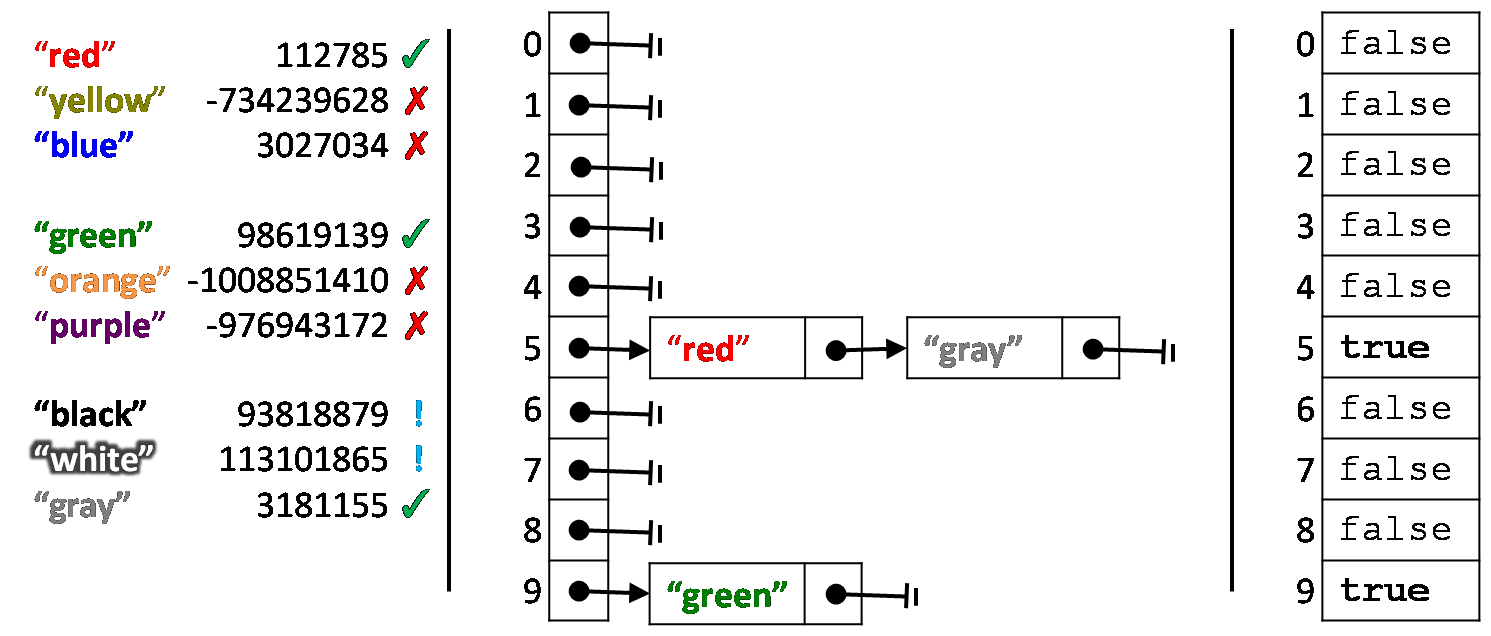
\includegraphics[trim=0 0 0 20, width=\textwidth]{img/bloom1.png}
\end{center}
\begin{quote}
\caption{On the left, some strings and their hash values according to
  the \lstinline'hash_mul31' hash function.}
\label{fig:badbloom}

\medskip

  In the middle,  a separate-chaining hash table using this hash function,
  after the insertion of the strings \lstinline'"green"', \lstinline'"red"',
  and \lstinline'"gray"'.  Next to them is an indication of whether the Bloom
  filter (first implementation) returns a true positive
  (\textcolor{Green}{\ding{52}}), a false positive
  (\textcolor{cyan}{\bf !}), or a (true) negative (\textcolor{Red}{\ding{56}}).

\medskip

  On the right, a Bloom filter (first implementation) using this hash
  function, after the insertion of the strings \lstinline'"green"',
  \lstinline'"red"', and \lstinline'"gray"'.
\end{quote}
}}
\end{figure}

In the example from Figure~\ref{fig:badbloom}, we would give false
positives for \lstinline'"white"' and \lstinline'"black"', since
those strings collide with strings that are in the set. We would
correctly return \lstinline'false' when asked if other strings, like
\lstinline'"yellow"', were in the set.

\begin{task}[7]
\TAGS{ds-invariant, hashing, set}
In the file \lstinline'bloom1.c0', implement Bloom filters according
to the description above. The type \lstinline'bloom_t' should be a
\lstinline'struct bloom_filter*':
\begin{quote}
\begin{lstlisting}
struct bloom_filter {
    bool[] data;
    int capacity;   // capacity == \length(data)
};
\end{lstlisting}
\end{quote}
You must write and correctly use a data structure invariant
\lstinline'is_bloom(B)'. Calling the constructor
\lstinline'bloom_new('$m$\lstinline')' should create a Bloom filter whose
array has size $m$. The Bloom filter must use the hash function
\lstinline'hash_mul31' that you implemented in lab, and must compute the hash
index from the hash value by modding by the size of the table and then taking
the absolute value.
\end{task}

\bigskip
This implementation of the Bloom filter interface uses much less space
than an actual hash table. An empty basic Bloom filter with table size
$m$ uses one-eighth of the space that the corresponding empty hash
table uses. While a hash table has to allocate more space for every
element, the basic Bloom filter never allocates any additional space.

\section{Better Bloom Filters}

In this section, we'll discuss and then implement two improvements to
our Bloom filters.

\subsection{Multiple Hash Functions}
\label{sec:multihash}

It's inevitable to have  collisions in a hash table; we
tolerate these collisions because they only make the hash table a
little bit slower. In Bloom filters, however, collisions cause us to
get false positives. It's worth going to greater lengths to avoid this.

\begin{figure}
\fbox{%
\parbox{\linewidth}{%
\begin{center}
  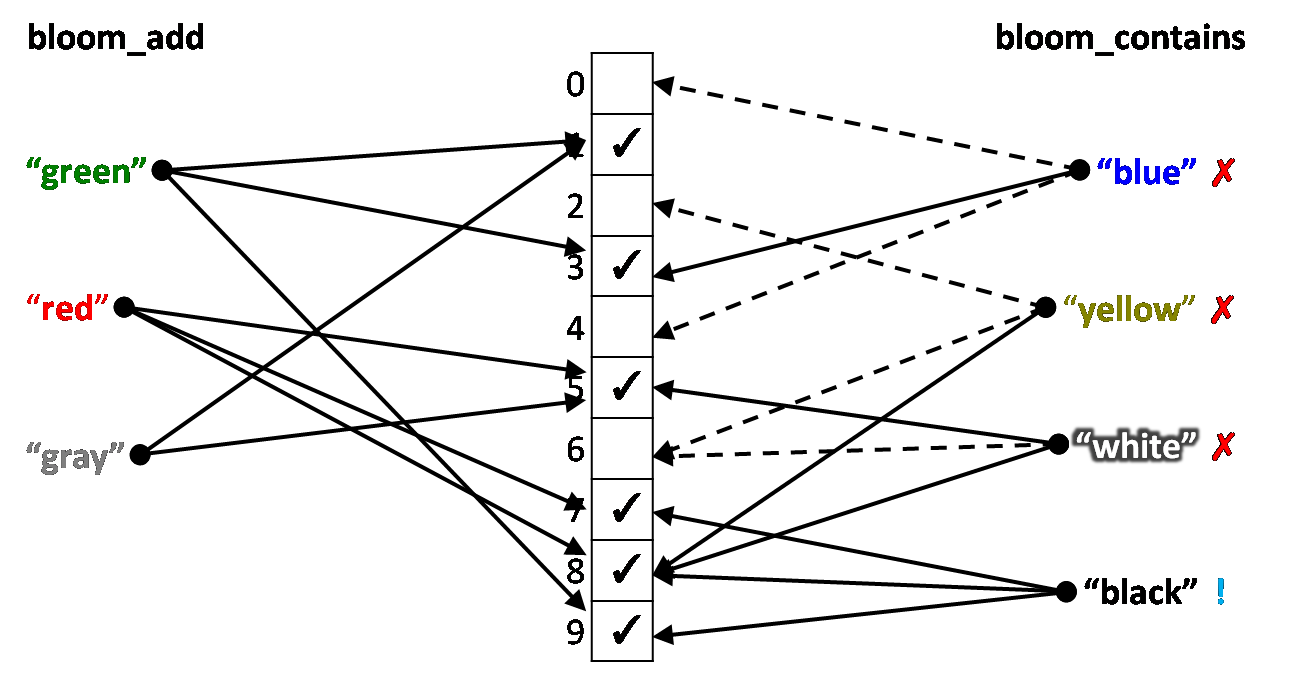
\includegraphics[width=\textwidth]{img/bloom2.png}
\end{center}
\begin{quote}
\caption{A Bloom filter using multiple hash functions.}
\label{fig:betterbloom}
\end{quote}
\vspace{-4ex}
}}
\end{figure}

Increasing $m$, the size of the table, will help some. However, this strategy
only takes us so far. Another remarkably effective strategy is implementing
\emph{multiple} hash functions, and inserting each item with \emph{every}
available hash functions. This means that more of the hash table gets filled
up with \lstinline'true' values (represented as checkmarks in
Figure~\ref{fig:betterbloom}). When we test whether an element is in the hash
table, then we check all of the indices where that element should hash. If any
of them are \lstinline'false', we can conclude that the element was never
added to the hash table.

The mathematics of why this works better than just growing the array
will be a topic for future courses (including Computational Discrete
Mathematics, Probability and Computing, and Algorithms). Looking at
Figure~\ref{fig:betterbloom}, we see the result of putting our example
strings into a Bloom filter. In that figure, the three hash indices we
pick are the last three digits of the \lstinline'hash_mul31' hash
values that we saw in Figure~\ref{fig:badbloom}. In your
implementation, you will want to use three entirely different hash
functions.

While we still have a false positive for the string
\lstinline'"black"', the Bloom filter has fewer false positives than
before.

\begin{task}[3]
\TAGS{hashing, randomness}
In the file \lstinline'bloom2.c0', implement three hash functions,
\lstinline'hash1(s)', \lstinline'hash2(s)', and \lstinline'hash3(s)',
which take strings and return integers. These will be the three hash
functions used by your improved Bloom filter. At most one should be
the \lstinline'hash_mul31' function from lab.
\end{task}


\subsection{Packing Bits}
\label{sec:bitpacking}

The smallest unit of memory that our computer can efficiently work
with is called a \emph{byte}. On most of our modern computers, a
value of the \lstinline'bool' type takes up 1 byte, a value of the
\lstinline'int' type takes up 4 bytes, and an address (the value of a
pointer or an array) takes up 8 bytes. That's why we said that an
empty Bloom filter used about one-eighth of the memory that an empty
hash table of the same size used.

Recall that our 32-bit integers are made up of 32 bits, each of which
are potentially 1 or 0. A \lstinline'bool[]' needs to use $m$ bytes to
represent $m$ \lstinline'true' or \lstinline'false' values. On the
other hand, an \lstinline'int[]' \lstinline'A' can store 32
\lstinline'true' or \lstinline'false' values in the 32 bits of
\lstinline'A[0]', 32 more \lstinline'true' or \lstinline'false' values
in the 32 bits of \lstinline'A[1]', and so on. An integer array that
needs to store $m$ true/false values (bits) needs to only have $\lceil
m / 32 \rceil$ integers, which takes up $4 \times \lceil m / 32
\rceil$ bytes. This is another 8-fold improvement in our memory usage!

\begin{task}[2]
\TAGS{array, bit-patterns, safety}
In the file \lstinline'bloom2.c0', implement two functions which
facilitate treating an array of $n$ integers as an array of $32n$
Boolean values:
\begin{quote}
\begin{lstlisting}
bool get_bit(int[] A, int i)
  /*@requires 0 <= i && i/32 < \length(A); @*/ ;

void set_bit(int[] A, int i)
  /*@requires 0 <= i && i/32 < \length(A); @*/
  /*@ensures get_bit(A, i); @*/ ;
\end{lstlisting}
\end{quote}
\end{task}
Using \lstinline'get_bit' and \lstinline'set_bit' should allow you
to treat \lstinline'A' like a \lstinline'bool[]' that is 32 times
longer than \length{(A)}. The function call
\lstinline'get_bit(A, i)' should have the same result that the
expression \lstinline'A[i]' would have for the \lstinline'bool[]'. The
function call \lstinline'set_bit(A, i)' should have the same result
that the statement \lstinline'A[i] = true;' would have for the
\lstinline'bool[]'.

For a freshly-allocated integer array, \lstinline'get_bit(A, i)'
should return \lstinline'false' for any valid
\lstinline'i'. Subsequent calls to \lstinline'set_bit(A, i)' turn
single bits of the array to \lstinline'true' (or leave them alone if
they are already set).

The exact way that you store 32 \lstinline'true'/\lstinline'false' values
within an integer is up to you, but it should be similar to the way you stored
four 8-bit intensity values in the Pixels assignment. Your approach should be
relatively simple and should be documented with comments.


\subsection{Implementation}

\begin{task}[7]
\TAGS{bit-patterns, ds-invariant, hashing, set}
In the file \lstinline'bloom2.c0', implement Bloom filters incorporating
the aforementioned improvements. The type
\lstinline'bloom_t' should be a \lstinline'struct bloom_filter*':
\begin{quote}
\begin{lstlisting}
struct bloom_filter {
    int[] data;
    int limit; // limit == \length(data)
};
\end{lstlisting}
\end{quote}
You must write and correctly use a data structure invariant
\lstinline'is_bloom(B)'. Calling the constructor
\lstinline'bloom_new('$n$\lstinline')' should create a Bloom filter
whose data field is an array of $\lceil n / 32 \rceil$ integers. This
means that the effective table size will always be a multiple of 32.
The effective table size will be $32 \times \lceil n / 32 \rceil$, which is
between 0 and 31 (inclusive) bits bigger than the requested table size.

Use the three hash functions you implemented in
Section~\ref{sec:multihash} as your three hash functions. The data
structure should only need to access and manipulate the
\lstinline'data' array using the \lstinline'get_bit' and
\lstinline'set_bit' functions from Section~\ref{sec:bitpacking}.
\end{task}

\end{document}

\section{Applications}

We're still not going to implement bloom filters yet! Instead, we're going
to write some applications.

\subsection{One-hit wonders}

One use of Bloom filters is \emph{caching}:

\begin{task}[2]
\TAGS{complexity, hashing, queue, set}
In the file \lstinline'applications.c0', implement the following
function. It should use the Bloom filter interface to take in a queue
of strings and store in the set all the inputs that are mentioned
\emph{multiple times}
\begin{quote}
\begin{lstlisting}
set_t frequently_accessed_inputs(queue_t inputs)
  /*@requires inputs != NULL; @*/
  /*@ensures \result != NULL; @*/ ;
\end{lstlisting}
\end{quote}
\end{task}


\end{document}
